\subsubsection{NASA-TLX}
\label{subsubsec:results_nasa_tlx_1}

The NASA-TLX provides two relevant pieces of information to the workload analysis. The first is the score attributed to the "mental demand" dimension and the second is the average obtained from NASA-TLX's six dimensions. The two analyses are presented in the next subsections.

\paragraph*{Analysis of the mental demand scale}\mbox{}\\


Figure \ref{fig:boxplot_md_blind_scene}  presents a boxplot of the mental demand score grouped by the methods. This figure shows that there may be two groups: one associated with lower demand, composed of base and audio, and another with higher demand, composed of haptic belt, virtual cane and mixture. It indicates that maybe a guidance method that uses vibration as input is not intuitive. Figure \ref{fig:boxplot_md_blind_rounds} presents a boxplot of the mental demand grouped by the rounds, confirming the general tendency to reduce the required "mental demand". 

\begin{figure}[!htb]
    \centering
    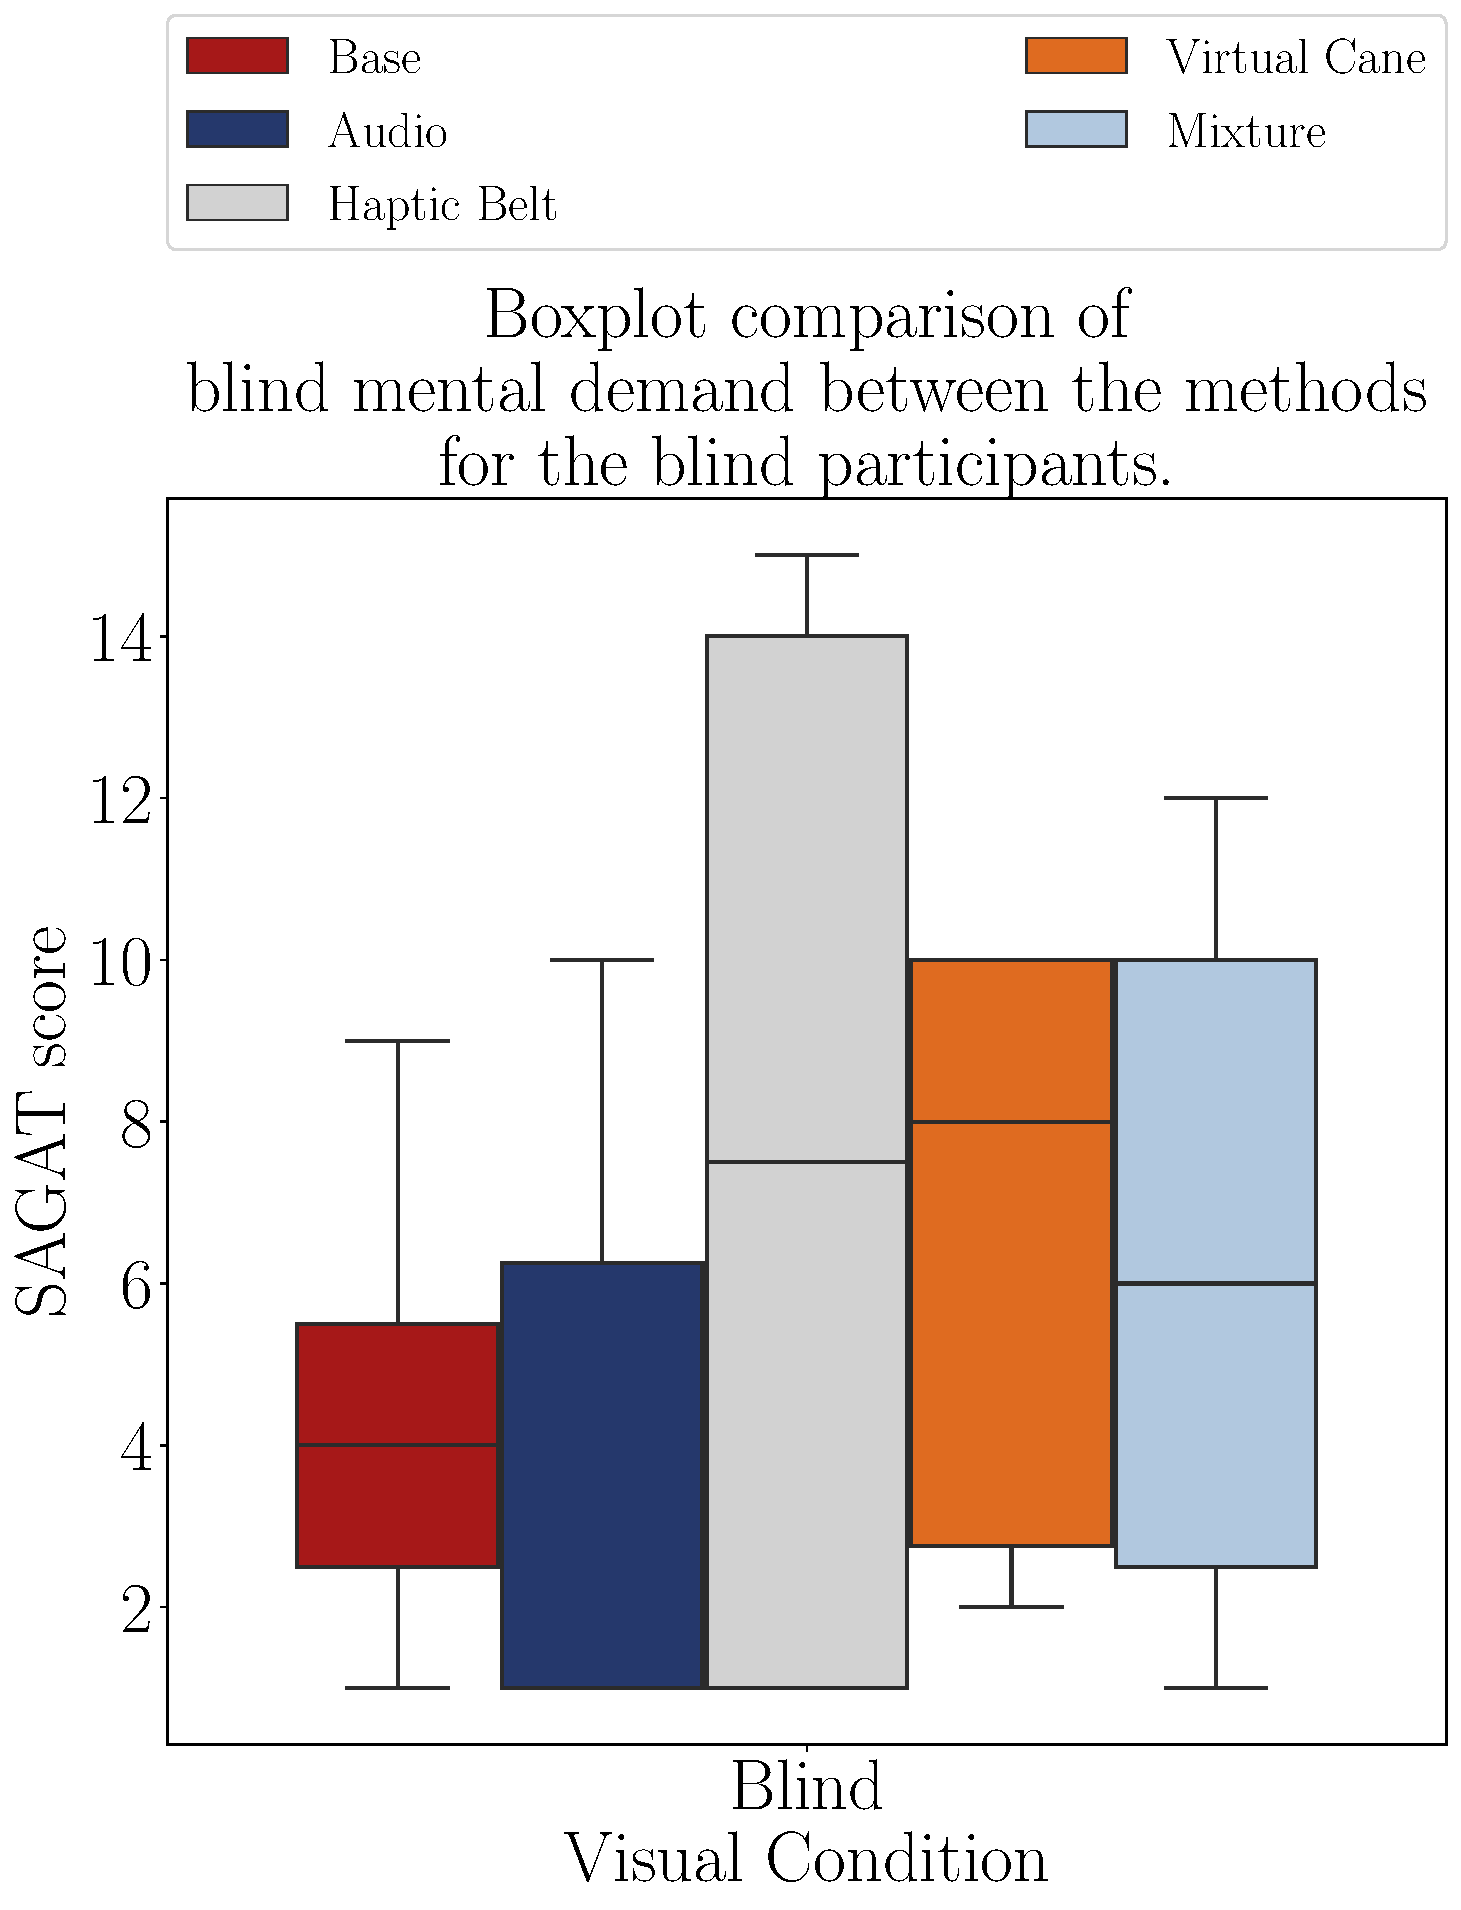
\includegraphics[width = 0.75\linewidth]{3 - Resultados/Figuras/boxplot_md_blind_scene.pdf}
    \caption{Boxplot of the mental demand of the blind participants grouped by the methods.}
    \label{fig:boxplot_md_blind_scene}
\end{figure}    
\begin{figure}[!htb]
    \centering
    %\vspace{3ex}
    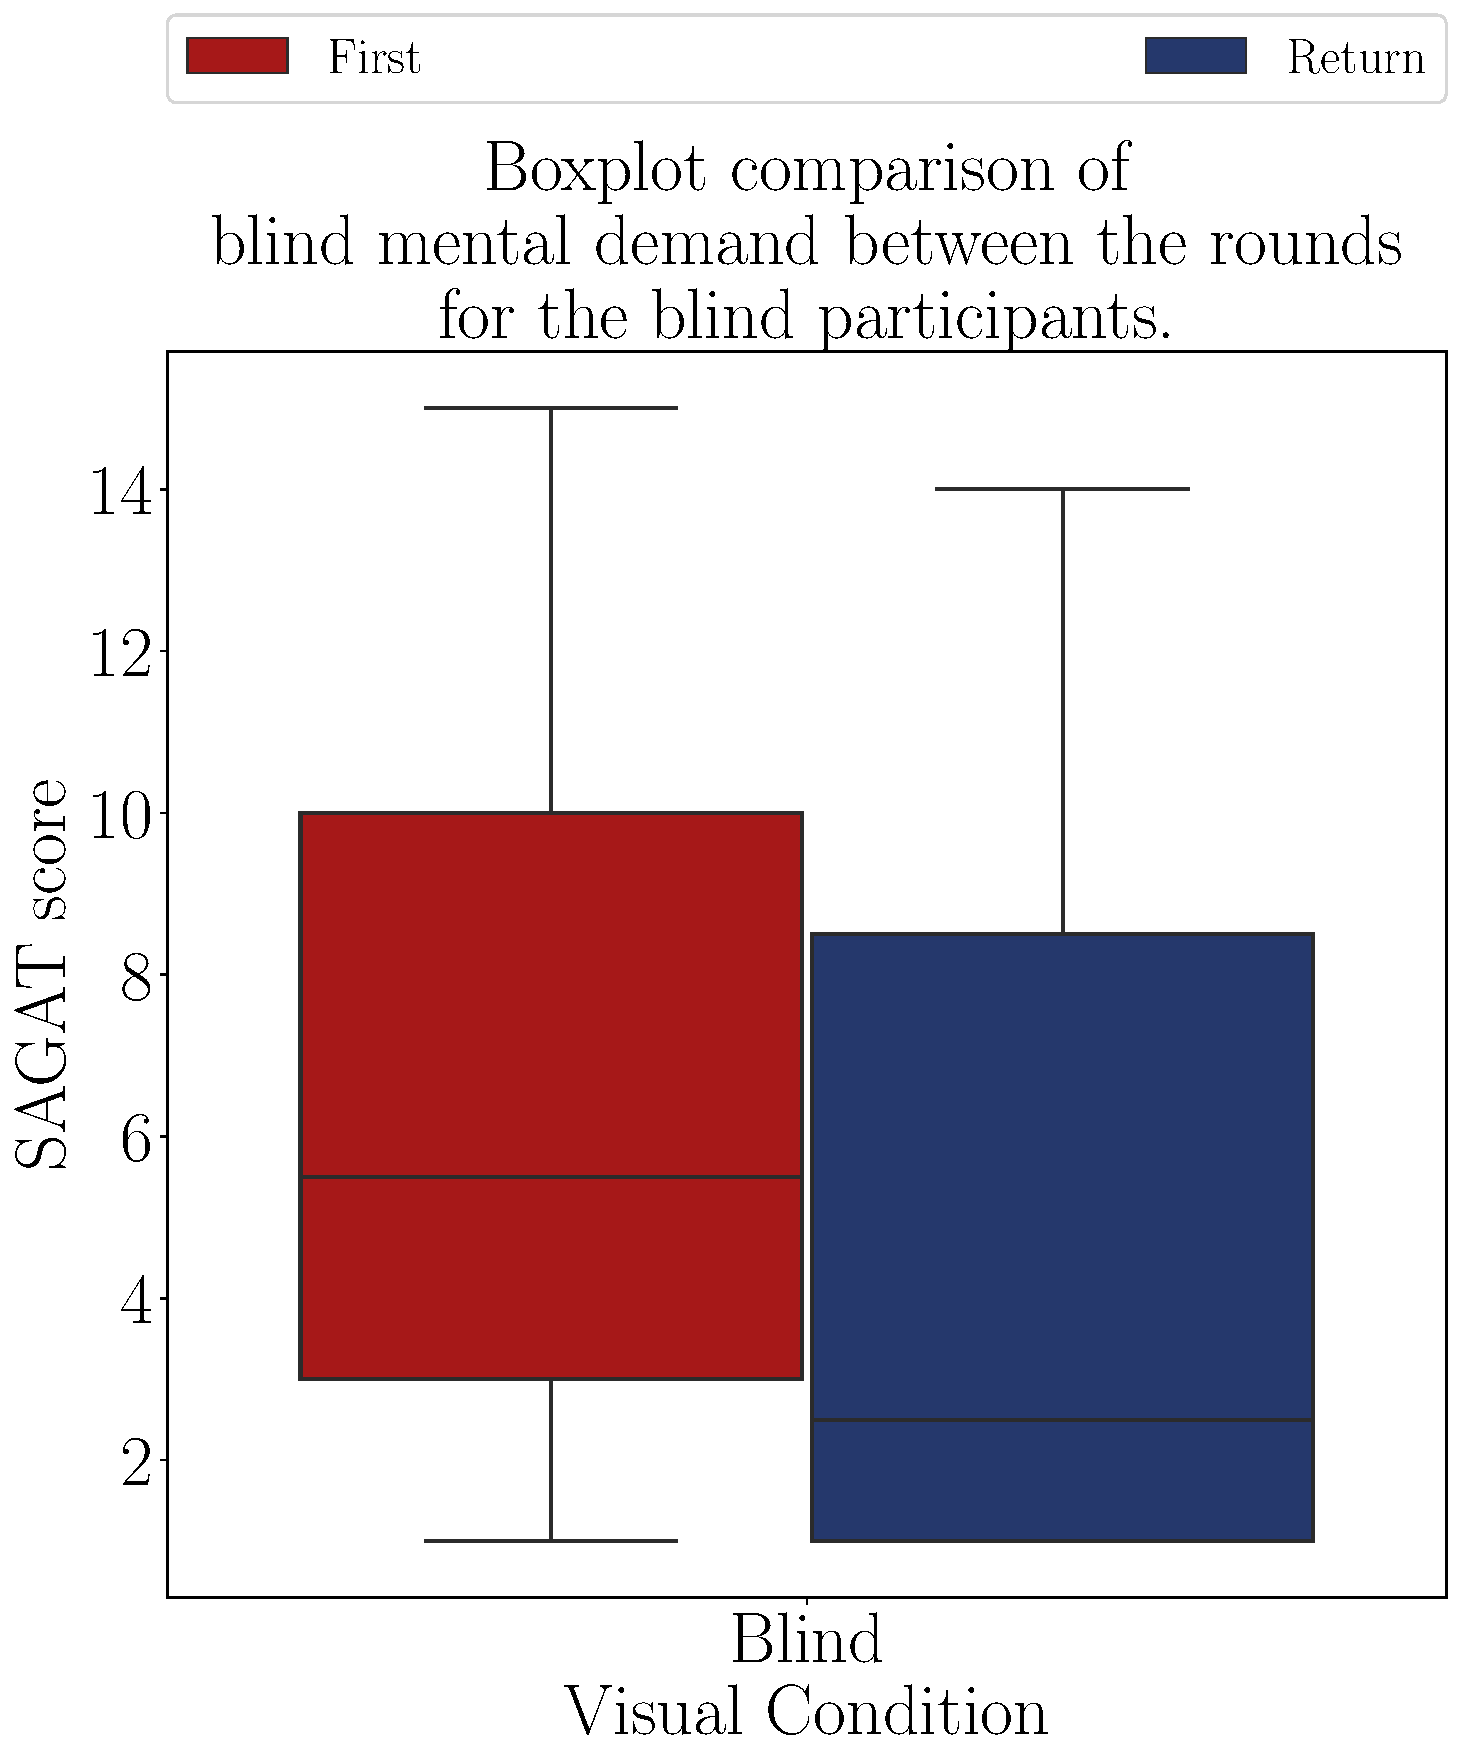
\includegraphics[width = 0.75\linewidth]{3 - Resultados/Figuras/boxplot_md_blind_rounds.pdf}
    \caption{Boxplot of the mental demand of the blind participants grouped by the rounds.}
    \label{fig:boxplot_md_blind_rounds}
\end{figure}

The results of ANOVA are presented in Table \ref{tab:blocanova_md_avg_two_way_blind}. A p-value of 0.05 is commonly adopted as a threshold to confirm the hypothesis. According to this criterion, neither method or round have a significant influence on the mental demand.


\begin{table}[!htb]
\centering
\caption{ANOVA p-value for mental demand -- blind participants}
\label{tab:blocanova_md_avg_two_way_blind}
\begin{tabular}{ll}
\toprule
          Source & P-Value \\
\midrule
    \    Methods &   0.170 \\
     \    Rounds &   0.075 \\
\    Interaction &   0.993 \\
\bottomrule
\end{tabular}
\end{table}



\paragraph*{Analysis of the NASA-TLX score}\mbox{}\\

Figure \ref{fig:boxplot_nasa_blind_scene} presents the boxplot with the NASA-TLX global score grouped by the methods. Similar to what happened for the "mental demand", it is possible to split the methods into two different groups: base and audio, which require a lower level of workload, and another group, which requires a higher level. Figure \ref{fig:boxplot_nasa_blind_rounds} presents a boxplot with the NASA-TLX global score grouped by the rounds, showing that the two groups are still different. 

\begin{figure}[!htb]
    \centering
    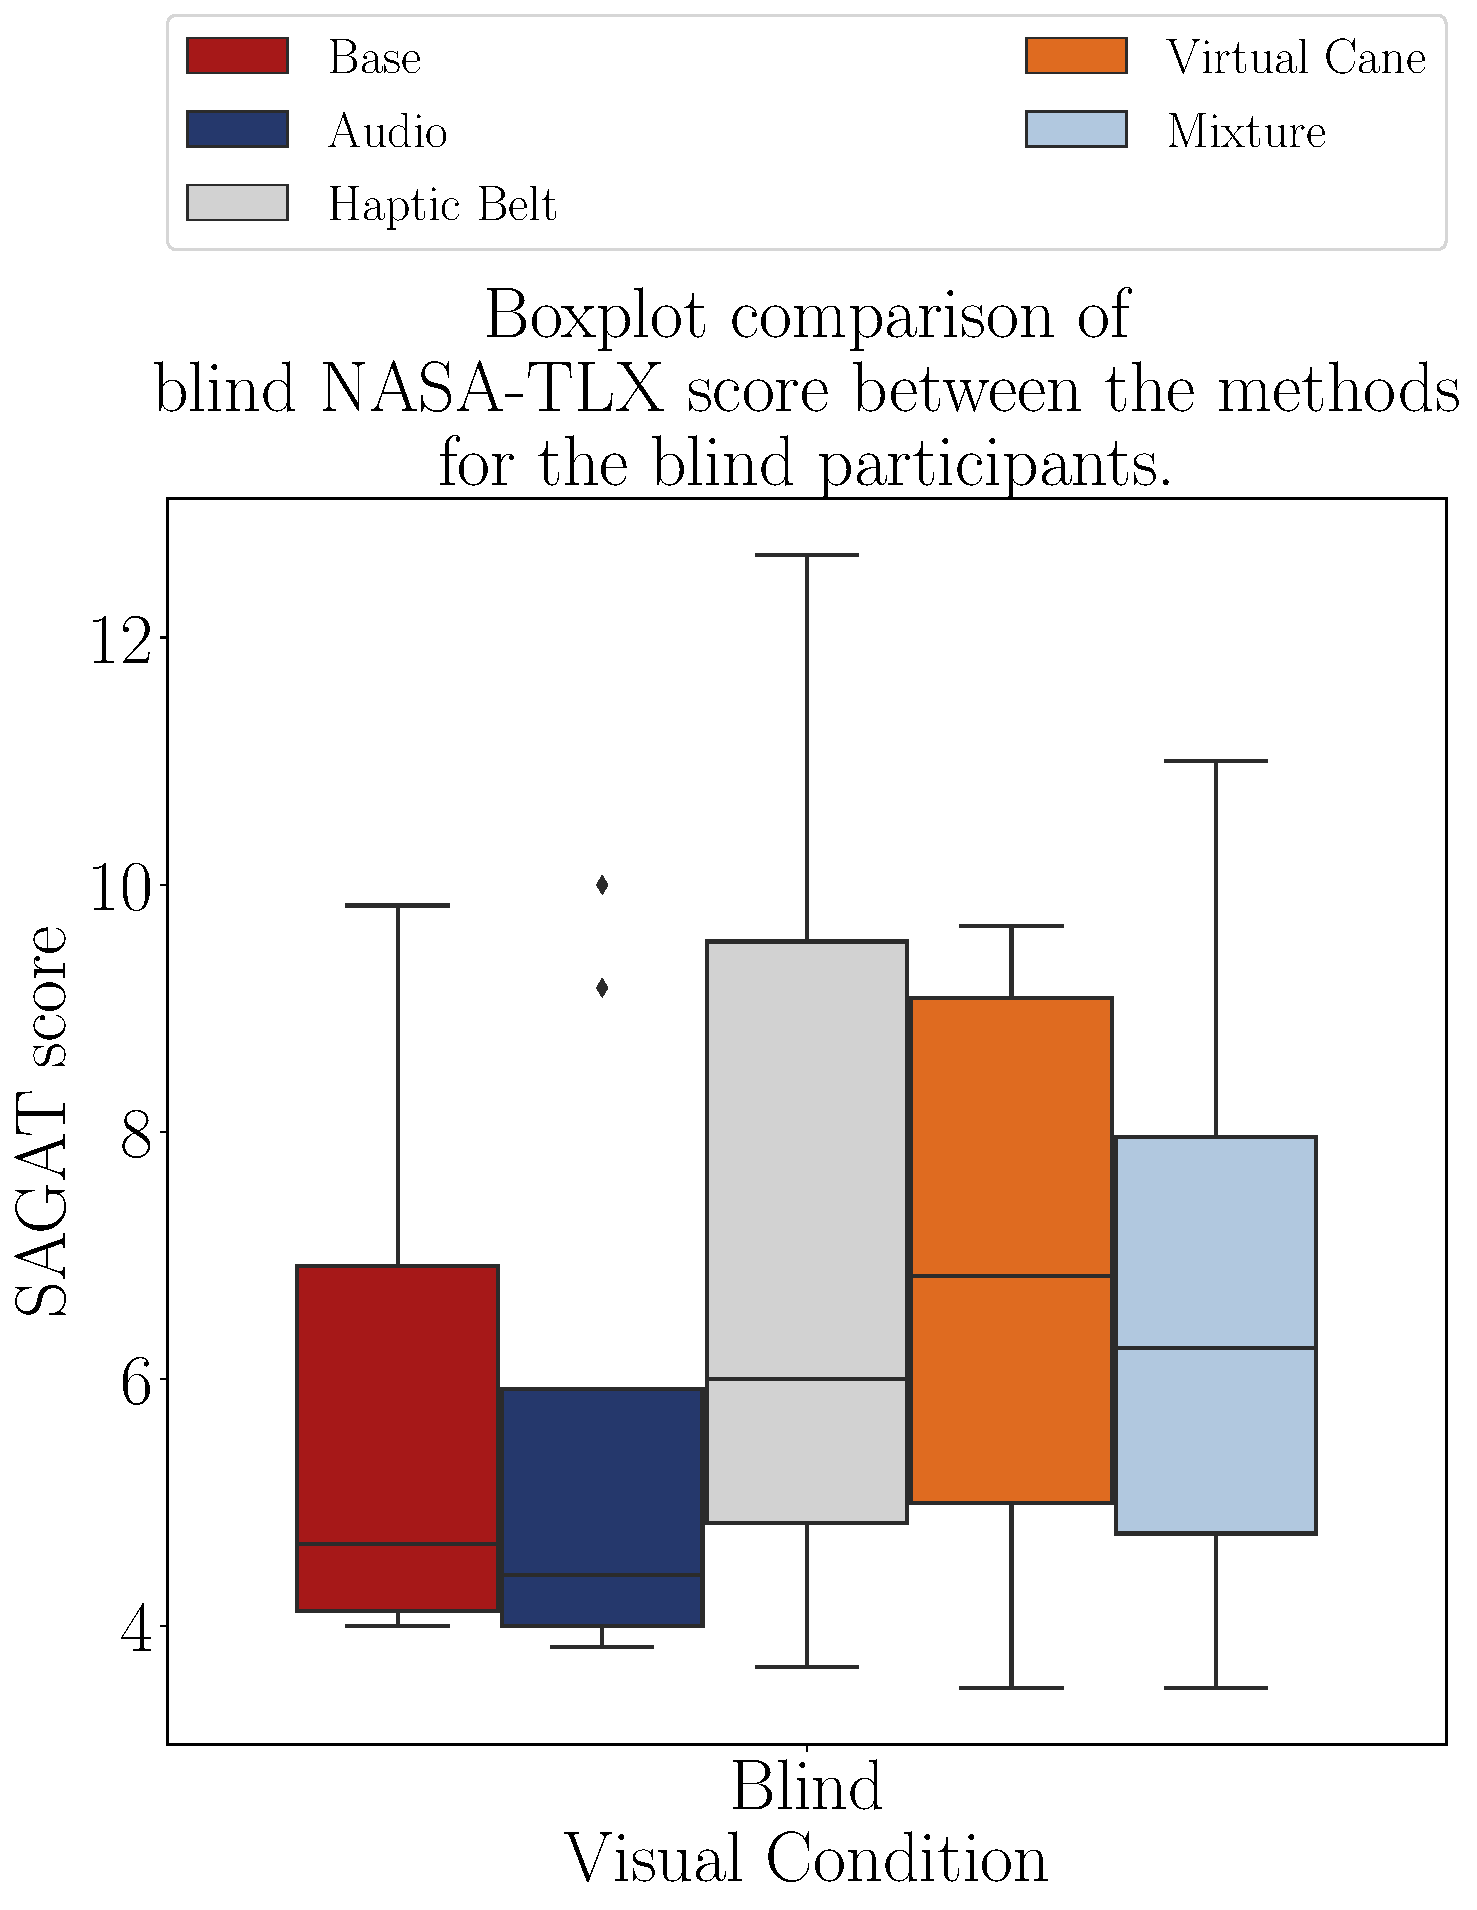
\includegraphics[width = 0.75\linewidth]{3 - Resultados/Figuras/boxplot_nasa_blind_scene.pdf}
    \caption{Boxplot of the mental demand of the blind participants grouped by the methods.}
    \label{fig:boxplot_nasa_blind_scene}
\end{figure}    
\begin{figure}[!htb]
    \centering
    %\vspace{3ex}
    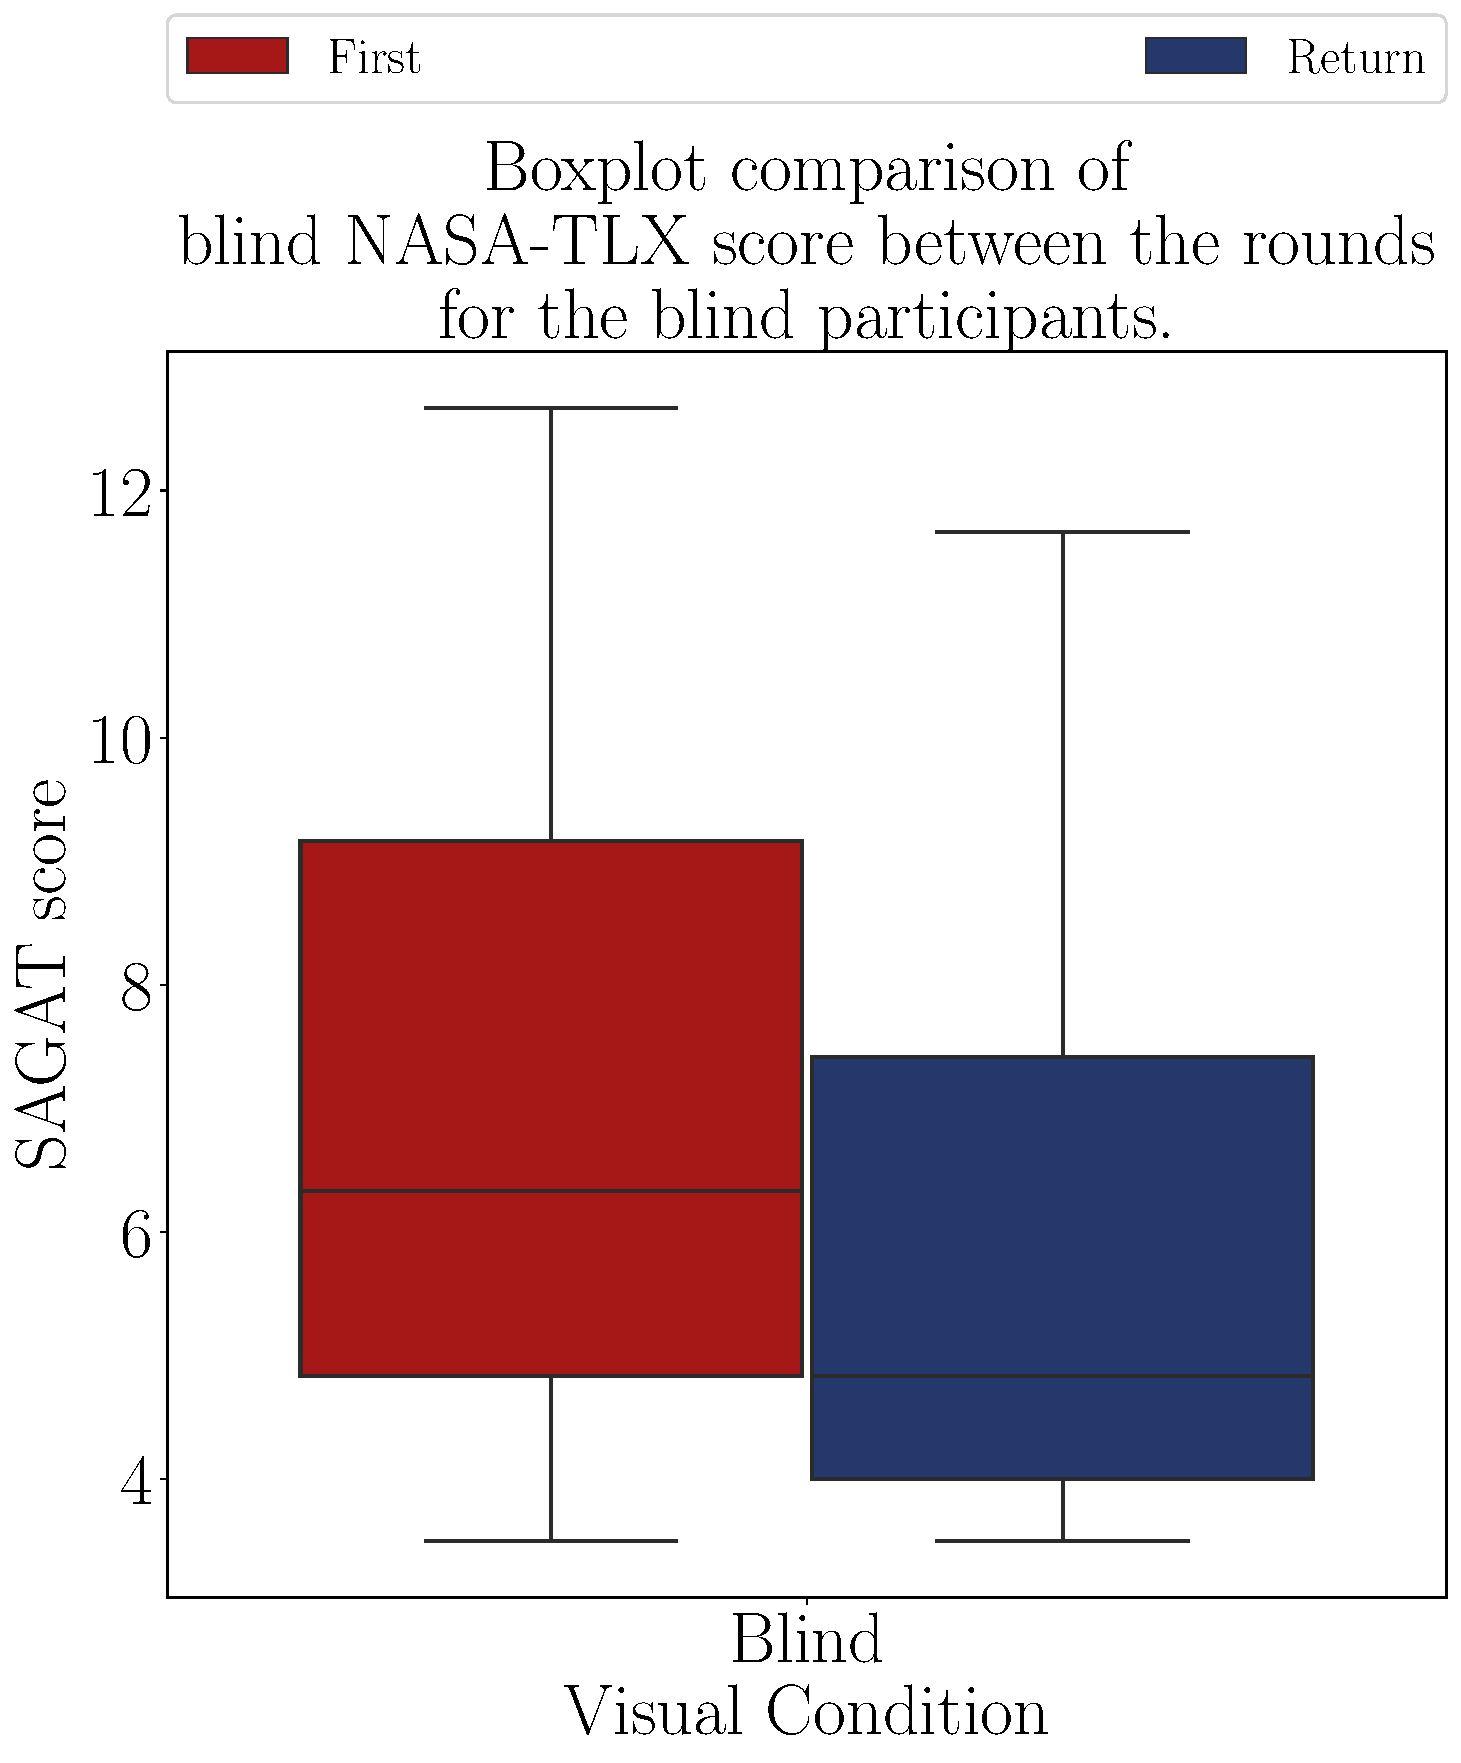
\includegraphics[width = 0.75\linewidth]{3 - Resultados/Figuras/boxplot_nasa_blind_rounds.pdf}
    \caption{Boxplot of the mental demand of the blind participants grouped by the rounds.}
    \label{fig:boxplot_nasa_blind_rounds}
\end{figure}

The sample residuals are not homogeneous meaning that the participants have different variability among them and that impacts the ANOVA.

Table \ref{tab:blocanova_nasa_avg_two_way_blind} brings the p-value resulting from ANOVA. In this case, both the methods and the rounds were appointed as significant variables that influence the mean value of the NASA-TLX global score. 


\begin{table}[!htb]
\centering
\caption{Anova p-value for the NASA-TLX score -- blinded users.}
\label{tab:blocanova_nasa_avg_two_way_blind}
\begin{tabular}{lrrrrl}
\toprule
          Source & P-Value \\
\midrule
    \    Methods & 0.029** \\
     \    Rounds & 0.022** \\
\    Interaction &   0.814 \\
\bottomrule
\end{tabular}
\end{table}



Finally a pairwise Fisher LSD test comparing each pair of guidance methods. The results show that only audio is similar to the base. All the other methods are different from each other.